\documentclass[aspectratio=169]{beamer}
\usetheme{Madrid}
\usecolortheme{default}

% Packages
\usepackage{graphicx}
\usepackage{listings}
\usepackage{xcolor}
\usepackage{hyperref}
\usepackage{amsmath}
\usepackage{booktabs}
\usepackage{multirow}

% Code styling
\lstset{
    language=Python,
    basicstyle=\tiny\ttfamily,
    keywordstyle=\color{blue},
    commentstyle=\color{green!60!black},
    stringstyle=\color{red},
    numbers=left,
    numberstyle=\tiny,
    stepnumber=1,
    numbersep=5pt,
    frame=single,
    breaklines=true,
    showstringspaces=false
}

% Title information
\title[Phân tích Dữ liệu Streaming Thời gian Thực]{Phân tích Dữ liệu Streaming Thời gian Thực\\với Apache Spark và Python}
\subtitle{Hệ thống Phân tích Kho lưu trữ GitHub}
\author{Shachak Rozenblat}
\institute{Mã số sinh viên: 216141459}
\date{\today}

\begin{document}

% Title slide
\frame{\titlepage}

% Table of contents
\begin{frame}{Mục lục}
    \tableofcontents
\end{frame}

% Section 1: Introduction
\section{Giới thiệu}

\begin{frame}{Tổng quan Dự án}
    \begin{itemize}
        \item \textbf{Mục tiêu:} Phân tích dữ liệu kho lưu trữ GitHub theo thời gian thực
        \item \textbf{Kiến trúc:} Hệ thống microservices ba tầng
        \item \textbf{Công nghệ:} Apache Spark, Python, Flask, Redis, Docker
        \item \textbf{Nguồn dữ liệu:} GitHub API (kho lưu trữ Python, Java, JavaScript)
        \item \textbf{Xử lý:} Streaming micro-batch 60 giây
        \item \textbf{Đầu ra:} Bảng điều khiển web tương tác với biểu đồ trực quan
    \end{itemize}
    
    \vspace{0.5cm}
    \begin{block}{Tính năng chính}
        \begin{itemize}
            \item Thu thập dữ liệu thời gian thực từ GitHub API
            \item Xử lý stream phân tán với Spark
            \item 8 tác vụ phân tích khác nhau
            \item Triển khai container hóa với Docker Compose
        \end{itemize}
    \end{block}
\end{frame}

% Section 2: System Architecture
\section{Kiến trúc Hệ thống}

\begin{frame}{Tổng quan Kiến trúc Hệ thống}
    \begin{center}
        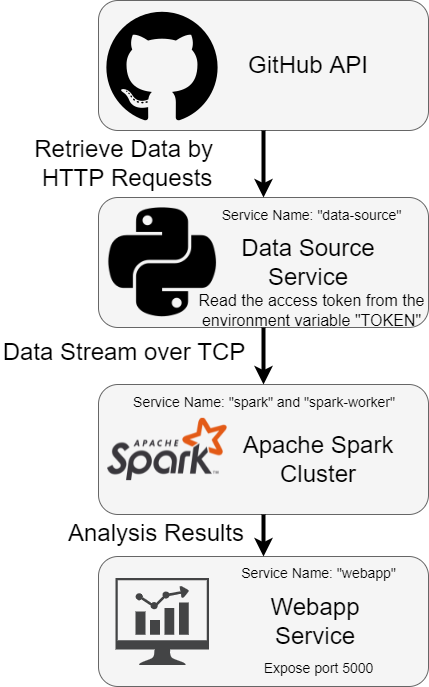
\includegraphics[width=0.8\textwidth]{System_Architecture.png}
    \end{center}
    
    \vspace{0.3cm}
    \begin{columns}
        \column{0.5\textwidth}
        \textbf{Luồng Dữ liệu:}
        \begin{enumerate}
            \item GitHub API
            \item Dịch vụ Nguồn Dữ liệu
            \item Spark Streaming
            \item Ứng dụng Web
            \item Bảng điều khiển Frontend
        \end{enumerate}
        
        \column{0.5\textwidth}
        \textbf{Đặc điểm chính:}
        \begin{itemize}
            \item Kiến trúc microservices
            \item Triển khai container hóa
            \item Xử lý thời gian thực
            \item Thiết kế chịu lỗi
        \end{itemize}
    \end{columns}
\end{frame}

\begin{frame}{Kiến trúc Thành phần}
    \begin{columns}
        \column{0.5\textwidth}
        \textbf{1. Dịch vụ Nguồn Dữ liệu}
        \begin{itemize}
            \item Python 3.9
            \item Truy vấn GitHub API
            \item Khoảng thời gian 15 giây
            \item Máy chủ TCP socket (cổng 9999)
            \item Stream dữ liệu JSON
        \end{itemize}
        
        \vspace{0.3cm}
        \textbf{2. Cụm Apache Spark}
        \begin{itemize}
            \item Nút Master + Worker
            \item Khoảng thời gian batch 60 giây
            \item Xử lý micro-batch
            \item Bật checkpointing
        \end{itemize}
        
        \column{0.5\textwidth}
        \textbf{3. Ứng dụng Web}
        \begin{itemize}
            \item Flask (Python)
            \item RESTful API
            \item Biểu đồ Matplotlib
            \item Cổng 5000
        \end{itemize}
        
        \vspace{0.3cm}
        \textbf{4. Redis Cache}
        \begin{itemize}
            \item Kho lưu trữ dữ liệu trong bộ nhớ
            \item Cache kết quả phân tích
            \item Cổng 6379
        \end{itemize}
        
        \vspace{0.3cm}
        \textbf{5. Bảng điều khiển Frontend}
        \begin{itemize}
            \item HTML/JavaScript
            \item Tự động làm mới (60s)
            \item Biểu đồ tương tác
        \end{itemize}
    \end{columns}
\end{frame}

% Section 3: Data Flow
\section{Luồng Dữ liệu}

\begin{frame}{Kiến trúc Luồng Dữ liệu}
    \begin{center}
        \Large
        \textbf{GitHub API} $\rightarrow$ \textbf{Nguồn Dữ liệu} $\rightarrow$ \textbf{TCP Socket} $\rightarrow$ \\
        \vspace{0.3cm}
        \textbf{Spark Streaming} $\rightarrow$ \textbf{HTTP POST} $\rightarrow$ \textbf{Webapp} $\rightarrow$ \\
        \vspace{0.3cm}
        \textbf{Redis} $\rightarrow$ \textbf{Bảng điều khiển Frontend}
    \end{center}
    
    \vspace{0.5cm}
    \begin{block}{Đặc điểm Thời gian}
        \begin{itemize}
            \item \textbf{Nguồn Dữ liệu:} Truy vấn GitHub API mỗi 15 giây
            \item \textbf{Spark Batch:} Xử lý dữ liệu mỗi 60 giây
            \item \textbf{Frontend:} Làm mới mỗi 60 giây
            \item \textbf{Độ trễ:} $\sim$60-75 giây từ GitHub push đến biểu đồ
        \end{itemize}
    \end{block}
\end{frame}

\begin{frame}{Giao tiếp Dịch vụ}
    \begin{table}[h]
        \centering
        \small
        \begin{tabular}{llll}
            \toprule
            \textbf{Từ} & \textbf{Đến} & \textbf{Giao thức} & \textbf{Cổng} \\
            \midrule
            GitHub API & Nguồn Dữ liệu & HTTPS & 443 \\
            Nguồn Dữ liệu & Spark & TCP Socket & 9999 \\
            Spark & Webapp & HTTP POST & 5000 \\
            Webapp & Redis & Redis Protocol & 6379 \\
            Frontend & Webapp & HTTP GET & 5000 \\
            \bottomrule
        \end{tabular}
    \end{table}
    
    \vspace{0.3cm}
    \begin{block}{Định dạng Dữ liệu}
        \begin{itemize}
            \item \textbf{Nguồn Dữ liệu $\rightarrow$ Spark:} JSON phân cách dòng mới (NDJSON)
            \item \textbf{Spark $\rightarrow$ Webapp:} JSON với 8 kết quả yêu cầu
            \item \textbf{Webapp $\rightarrow$ Frontend:} JSON với đường dẫn hình ảnh và dữ liệu
        \end{itemize}
    \end{block}
\end{frame}

% Section 4: Spark Processing
\section{Xử lý Spark}

\begin{frame}{Khởi tạo Streaming Context}
    \begin{lstlisting}[language=Python]
BATCH_INTERVAL = 60  # 60-second micro-batches
ssc = StreamingContext(sc, BATCH_INTERVAL)
ssc.checkpoint("checkpoint_EECS4415_Porject_3")

data = ssc.socketTextStream(
    "data-source", 9999,
    storageLevel=StorageLevel.MEMORY_AND_DISK
)
    \end{lstlisting}
    
    \vspace{0.3cm}
    \begin{block}{Tính năng chính}
        \begin{itemize}
            \item \textbf{Khoảng thời gian Batch:} 60 giây cho xử lý micro-batch
            \item \textbf{Checkpointing:} Cho phép chịu lỗi và khôi phục trạng thái
            \item \textbf{Mức lưu trữ:} MEMORY\_AND\_DISK để đảm bảo độ tin cậy
            \item \textbf{Nguồn Dữ liệu:} TCP socket stream từ dịch vụ data-source
        \end{itemize}
    \end{block}
\end{frame}

\begin{frame}{Pipeline Xử lý Dữ liệu}
    \begin{enumerate}
        \item \textbf{Nhận Text Stream}
        \begin{itemize}
            \item Nhận chuỗi JSON phân cách dòng mới
            \item Mỗi dòng = một đối tượng JSON kho lưu trữ
        \end{itemize}
        
        \item \textbf{Phân tích JSON}
        \begin{lstlisting}[language=Python, basicstyle=\tiny]
repos = data.flatMap(lambda json_str: [json.loads(json_str)])
        \end{lstlisting}
        
        \item \textbf{Xử lý RDD}
        \begin{lstlisting}[language=Python, basicstyle=\tiny]
repos.foreachRDD(processRdd)
        \end{lstlisting}
        
        \item \textbf{Xử lý Batch}
        \begin{itemize}
            \item Loại bỏ trùng lặp theo ID kho lưu trữ
            \item Quản lý trạng thái (toàn cục + theo batch)
            \item Thực thi 8 tác vụ phân tích
            \item Gửi kết quả đến webapp
        \end{itemize}
    \end{enumerate}
\end{frame}

\begin{frame}{Quản lý Trạng thái \& Loại bỏ Trùng lặp}
    \begin{block}{Trạng thái Toàn cục}
        \begin{itemize}
            \item \texttt{repositories}: Từ điển tất cả kho lưu trữ duy nhất theo ID
            \item \texttt{batch\_repositories}: Danh sách từ điển batch với timestamp
            \item Đảm bảo mỗi kho lưu trữ chỉ được đếm một lần trong toàn bộ stream
        \end{itemize}
    \end{block}
    
    \vspace{0.3cm}
    \begin{block}{Chiến lược Loại bỏ Trùng lặp}
        \begin{lstlisting}[language=Python, basicstyle=\tiny]
for repo in rdd.collect():
    if repo['id'] not in batch_repositories:
        batch_repositories[repo['id']] = repo
    if repo['id'] not in repositories:
        repositories[repo['id']] = repo
        \end{lstlisting}
    \end{block}
    
    \vspace{0.3cm}
    \begin{alertblock}{Đảm bảo}
        \begin{itemize}
            \item Yêu cầu 3.1, 3.3, 3.4: Mỗi repo được đếm chính xác một lần toàn cục
            \item Yêu cầu 3.2: Mỗi repo được đếm tối đa một lần mỗi batch 60 giây
        \end{itemize}
    \end{alertblock}
\end{frame}

% Section 5: Analytics Requirements
\section{Yêu cầu Phân tích}

\begin{frame}{Yêu cầu Cốt lõi (3.1-3.4)}
    \begin{block}{Yêu cầu 3.1: Tổng số Kho lưu trữ theo Ngôn ngữ}
        \begin{itemize}
            \item Đếm kho lưu trữ duy nhất theo ngôn ngữ
            \item Sử dụng Spark DataFrame \texttt{groupBy().count()}
            \item Mỗi kho lưu trữ được đếm chính xác một lần
        \end{itemize}
    \end{block}
    
    \begin{block}{Yêu cầu 3.2: Push Gần đây (60 Giây Cuối)}
        \begin{itemize}
            \item Đếm kho lưu trữ được push trong 60 giây cuối
            \item Lọc theo timestamp \texttt{pushed\_at}
            \item Dữ liệu chuỗi thời gian cho biểu đồ đường
        \end{itemize}
    \end{block}
    
    \begin{block}{Yêu cầu 3.3: Số Sao Trung bình theo Ngôn ngữ}
        \begin{itemize}
            \item Tính trung bình \texttt{stargazers\_count} theo ngôn ngữ
            \item Sử dụng tổng hợp Spark DataFrame
            \item Làm tròn đến 2 chữ số thập phân
        \end{itemize}
    \end{block}
    
    \begin{block}{Yêu cầu 3.4: Top 10 Từ Thường dùng}
        \begin{itemize}
            \item Trích xuất từ từ mô tả kho lưu trữ
            \item Sử dụng thao tác RDD: \texttt{flatMap}, \texttt{groupByKey}
            \item Tiền xử lý văn bản: chữ thường, loại bỏ ký tự không phải chữ cái
        \end{itemize}
    \end{block}
\end{frame}

\begin{frame}{Phân tích Nâng cao (3.5, 4.1-4.3)}
    \begin{block}{Yêu cầu 3.5: Mô hình Chủ đề (LDA)}
        \begin{itemize}
            \item Công nghệ: Spark MLlib LDA
            \item Quy trình: Tokenization $\rightarrow$ Loại bỏ từ dừng $\rightarrow$ TF-IDF $\rightarrow$ LDA
            \item Đầu ra: 5 chủ đề mỗi ngôn ngữ với từ khóa hàng đầu
            \item Mục đích: Xác định xu hướng công nghệ mới nổi
        \end{itemize}
    \end{block}
    
    \begin{block}{Yêu cầu 4.1: Nhận dạng Thực thể Được đặt tên}
        \begin{itemize}
            \item Công nghệ: Khớp mẫu dựa trên từ điển
            \item Danh mục: Công ty, Framework, Công cụ, Công nghệ
            \item Đầu ra: Top 5 thực thể mỗi danh mục mỗi ngôn ngữ
            \item Mục đích: Lập bản đồ hệ sinh thái công nghệ
        \end{itemize}
    \end{block}
    
    \begin{block}{Yêu cầu 4.2: Độ tương tự Cosine TF-IDF}
        \begin{itemize}
            \item Công nghệ: Spark MLlib TF-IDF + độ tương tự cosine thủ công
            \item Quy trình: Tiền xử lý văn bản $\rightarrow$ Vector TF-IDF $\rightarrow$ Độ tương tự cặp
            \item Đầu ra: Top 5 cặp kho lưu trữ tương tự nhất mỗi ngôn ngữ
            \item Mục đích: Xác định dự án liên quan, hệ thống đề xuất
        \end{itemize}
    \end{block}
    
    \begin{block}{Yêu cầu 4.3: Phân tích Chuỗi Thời gian}
        \begin{itemize}
            \item Công nghệ: Python datetime + Spark DataFrames
            \item Quy trình: Nhóm theo năm-tháng $\rightarrow$ Tính chỉ số $\rightarrow$ Tỷ lệ tăng trưởng
            \item Đầu ra: Xu hướng hàng tháng, tỷ lệ tăng trưởng, giai đoạn đỉnh
            \item Mục đích: Theo dõi tiến hóa công nghệ và dự báo xu hướng
        \end{itemize}
    \end{block}
\end{frame}

% Section 6: Implementation Details
\section{Chi tiết Triển khai}

\begin{frame}{Data Source Service}
    \begin{lstlisting}[language=Python, basicstyle=\tiny]
LANGUAGES = ['Python', 'Java', 'JavaScript']
TOKEN = "token" + os.getenv('TOKEN')

# TCP Socket Server
s.bind((HOST, PORT))
s.listen(1)
conn, addr = s.accept()

while True:
    for language in LANGUAGES:
        url = f'https://api.github.com/search/repositories?
              q=language:{language}&sort=updated&order=desc&per_page=50'
        response = requests.get(url, headers={"Authorization": TOKEN})
        repositories = response.json()["items"]
        
        for repository in repositories:
            if repository["language"] in LANGUAGES:
                json_data = f"{json.dumps(data)}\n".encode()
                conn.send(json_data)
    
    time.sleep(15)  # 15-second intervals
    \end{lstlisting}
    
    \begin{block}{Tính năng chính}
        \begin{itemize}
            \item Truy vấn GitHub API cho 3 ngôn ngữ tuần tự
            \item Tối đa 50 kho lưu trữ mỗi ngôn ngữ mỗi yêu cầu
            \item Stream dữ liệu JSON qua TCP socket
            \item Đọc PAT từ biến môi trường \texttt{TOKEN}
        \end{itemize}
    \end{block}
\end{frame}

\begin{frame}{Ứng dụng Web}
    \begin{columns}
        \column{0.5\textwidth}
        \textbf{Điểm cuối:}
        \begin{itemize}
            \item \texttt{POST /updateData}
            \begin{itemize}
                \item Nhận kết quả từ Spark
                \item Lưu vào Redis
            \end{itemize}
            \item \texttt{GET /getData}
            \begin{itemize}
                \item Lấy từ Redis
                \item Tạo biểu đồ
                \item Trả về JSON
            \end{itemize}
            \item \texttt{GET /}
            \begin{itemize}
                \item Phục vụ bảng điều khiển HTML
            \end{itemize}
        \end{itemize}
        
        \column{0.5\textwidth}
        \textbf{Biểu đồ:}
        \begin{itemize}
            \item \textbf{Yêu cầu 3.2:} Biểu đồ đường (chuỗi thời gian)
            \begin{itemize}
                \item Ba đường (một mỗi ngôn ngữ)
                \item Trục X: thời gian batch
                \item Trục Y: số lượng kho lưu trữ
            \end{itemize}
            \item \textbf{Yêu cầu 3.3:} Biểu đồ cột
            \begin{itemize}
                \item Trục X: ngôn ngữ lập trình
                \item Trục Y: số sao trung bình
            \end{itemize}
        \end{itemize}
    \end{columns}
    
    \vspace{0.3cm}
    \begin{block}{Công nghệ}
        Flask, Redis, Matplotlib, Frontend HTML/JavaScript
    \end{block}
\end{frame}

% Section 7: Deployment
\section{Triển khai}

\begin{frame}{Cấu hình Docker Compose}
    \begin{block}{Dịch vụ}
        \begin{itemize}
            \item \textbf{spark:} Nút Master (cổng 8080, 7077, 6066)
            \item \textbf{spark-worker:} Nút Worker (cổng 28081, 24040-24041)
            \item \textbf{data-source:} Dịch vụ Python (cổng 9999)
            \item \textbf{webapp:} Ứng dụng Flask (cổng 5000)
            \item \textbf{redis:} Dịch vụ Cache (cổng 6379)
        \end{itemize}
    \end{block}
    
    \vspace{0.3cm}
    \begin{block}{Các bước Triển khai}
        \begin{enumerate}
            \item Cấu hình biến môi trường \texttt{TOKEN} trong \texttt{docker-compose.yaml}
            \item Chạy \texttt{docker-compose up -d}
            \item Khởi chạy ứng dụng Spark:
            \begin{lstlisting}[language=bash, basicstyle=\tiny]
docker exec streaming-spark-1 /opt/spark/bin/spark-submit 
    /streaming/spark_app.py
            \end{lstlisting}
            \item Truy cập bảng điều khiển tại \texttt{http://localhost:5000}
        \end{enumerate}
    \end{block}
\end{frame}

\begin{frame}{Giám sát Hệ thống}
    \begin{columns}
        \column{0.5\textwidth}
        \textbf{Giao diện Web:}
        \begin{itemize}
            \item \textbf{Spark Master UI:} 
            \begin{itemize}
                \item \texttt{http://localhost:8080}
                \item Lập lịch công việc
                \item Phân bổ tài nguyên
            \end{itemize}
            \item \textbf{Spark Worker UI:}
            \begin{itemize}
                \item \texttt{http://localhost:28081}
                \item Thực thi tác vụ
            \end{itemize}
            \item \textbf{Spark Application UI:}
            \begin{itemize}
                \item \texttt{http://localhost:24040}
                \item Chỉ số streaming
            \end{itemize}
        \end{itemize}
        
        \column{0.5\textwidth}
        \textbf{Bảng điều khiển Web:}
        \begin{itemize}
            \item \texttt{http://localhost:5000}
            \item Biểu đồ thời gian thực
            \item Tự động làm mới mỗi 60 giây
            \item Hiển thị tất cả 8 kết quả yêu cầu
        \end{itemize}
        
        \vspace{0.3cm}
        \begin{alertblock}{Chịu lỗi}
            \begin{itemize}
                \item Checkpointing để khôi phục
                \item Lưu trữ MEMORY\_AND\_DISK
                \item Xử lý lỗi trong xử lý batch
            \end{itemize}
        \end{alertblock}
    \end{columns}
\end{frame}

% Section 8: Results
\section{Kết quả \& Biểu đồ}

\begin{frame}{Biểu đồ Bảng điều khiển}
    \begin{center}
        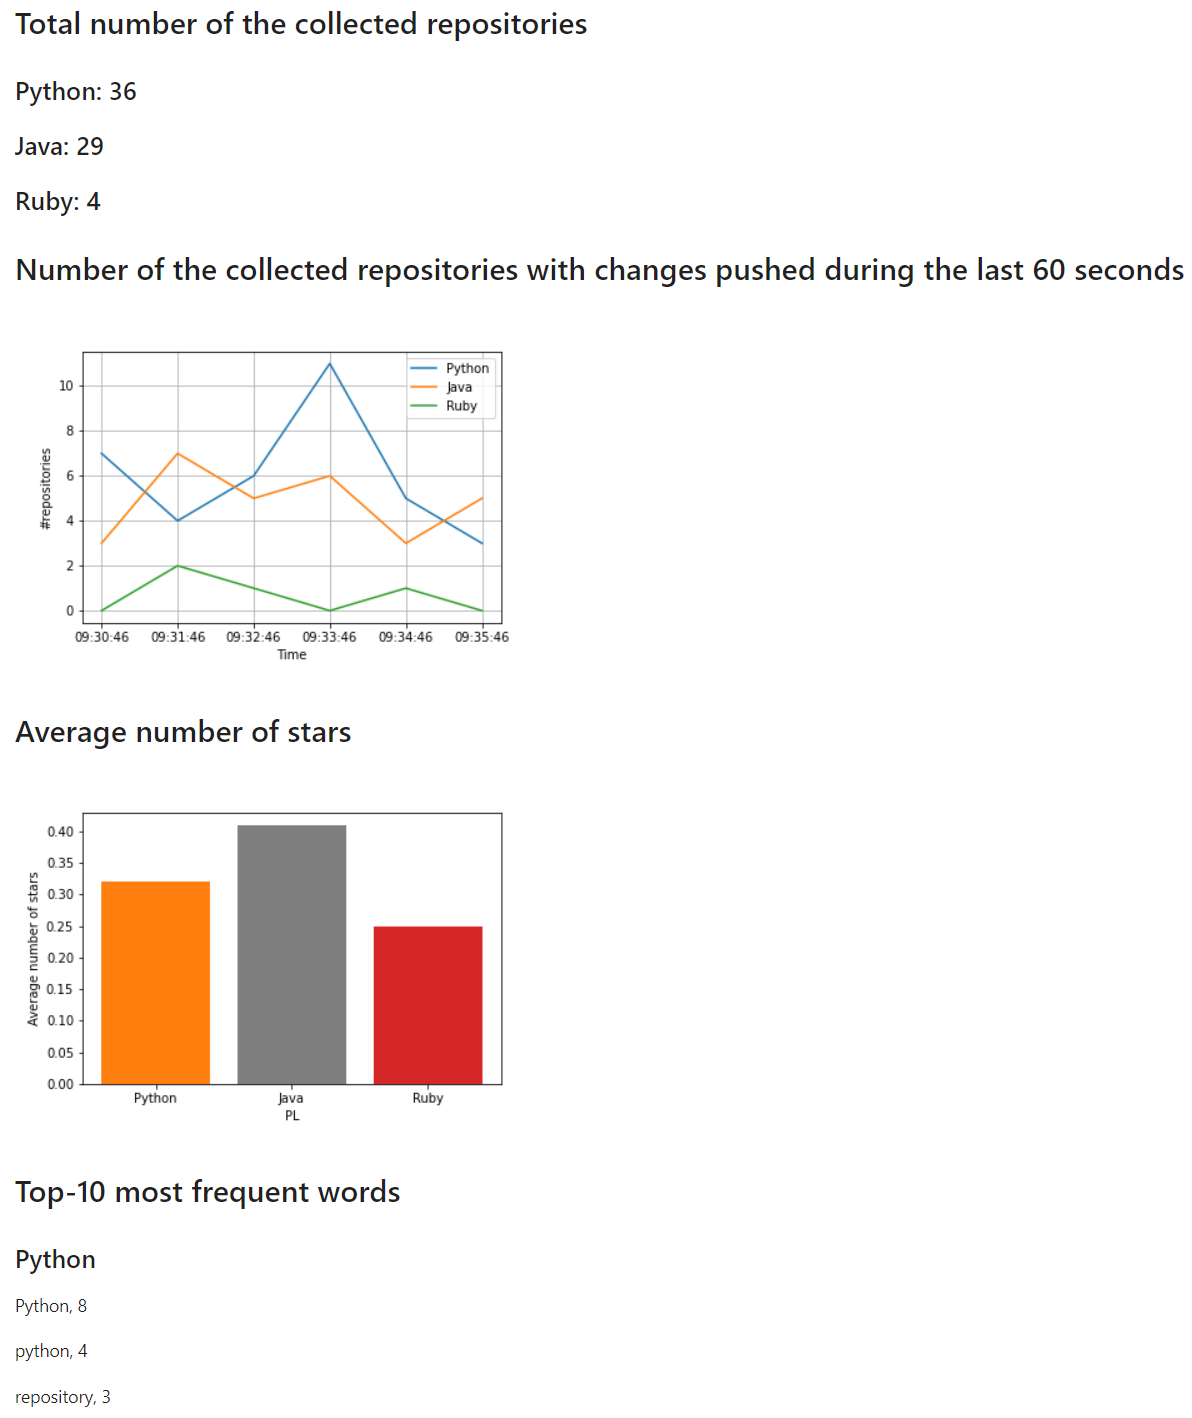
\includegraphics[width=0.7\textwidth]{Webapp.png}
    \end{center}
    
    \vspace{0.3cm}
    \begin{block}{Tính năng Bảng điều khiển}
        \begin{itemize}
            \item Cập nhật thời gian thực mỗi 60 giây
            \item Biểu đồ đường cho yêu cầu 3.2 (push gần đây theo thời gian)
            \item Biểu đồ cột cho yêu cầu 3.3 (số sao trung bình theo ngôn ngữ)
            \item Hiển thị văn bản cho yêu cầu 3.1, 3.4, và phân tích nâng cao
            \item Frontend JavaScript tương tác
        \end{itemize}
    \end{block}
\end{frame}

\begin{frame}{Kết quả Mẫu}
    \begin{block}{Yêu cầu 3.1: Tổng số Kho lưu trữ}
        \begin{itemize}
            \item Python: X kho lưu trữ
            \item Java: Y kho lưu trữ
            \item JavaScript: Z kho lưu trữ
        \end{itemize}
    \end{block}
    
    \begin{block}{Yêu cầu 3.3: Số Sao Trung bình}
        \begin{itemize}
            \item Python: X.XX sao trung bình
            \item Java: Y.YY sao trung bình
            \item JavaScript: Z.ZZ sao trung bình
        \end{itemize}
    \end{block}
    
    \begin{block}{Yêu cầu 3.4: Từ Hàng đầu}
        \begin{itemize}
            \item Python: ('framework', 45), ('library', 32), ...
            \item Java: ('application', 38), ('api', 29), ...
            \item JavaScript: ('react', 52), ('node', 41), ...
        \end{itemize}
    \end{block}
    
    \begin{block}{Phân tích Nâng cao}
        \begin{itemize}
            \item Mô hình Chủ đề: 5 chủ đề mỗi ngôn ngữ với từ khóa
            \item NER: Top công ty, framework, công cụ mỗi ngôn ngữ
            \item Độ tương tự: Cặp kho lưu trữ tương tự nhất
            \item Chuỗi Thời gian: Xu hướng hàng tháng và tỷ lệ tăng trưởng
        \end{itemize}
    \end{block}
\end{frame}

% Section 9: Key Features
\section{Tính năng chính \& Quyết định Thiết kế}

\begin{frame}{Quyết định Thiết kế chính}
    \begin{block}{Quản lý Trạng thái}
        \begin{itemize}
            \item \textbf{Lựa chọn:} Từ điển toàn cục Python
            \item \textbf{Lý do:} Đơn giản, hiệu quả cho streaming một driver
            \item \textbf{Đánh đổi:} Không phân tán; giảm nhẹ bằng checkpointing
        \end{itemize}
    \end{block}
    
    \begin{block}{Chiến lược Loại bỏ Trùng lặp}
        \begin{itemize}
            \item \textbf{Lựa chọn:} Loại bỏ trùng lặp dựa trên ID kho lưu trữ
            \item \textbf{Lý do:} Thời gian tra cứu O(1), triển khai đơn giản
            \item \textbf{Thực thi:} Áp dụng tại điểm thu thập trước khi phân tích
        \end{itemize}
    \end{block}
    
    \begin{block}{Batch vs. Xử lý Bản ghi}
        \begin{itemize}
            \item \textbf{Lựa chọn:} Xử lý micro-batch (khoảng 60 giây)
            \item \textbf{Lý do:} Cân bằng độ trễ với hiệu quả xử lý
            \item \textbf{Đánh đổi:} Không phải thời gian thực thực sự, nhưng cho phép phân tích phức tạp
        \end{itemize}
    \end{block}
    
    \begin{block}{Sử dụng DataFrame vs. RDD}
        \begin{itemize}
            \item \textbf{Lựa chọn:} Phương pháp hỗn hợp
            \item \textbf{Lý do:} DataFrame cho tổng hợp, RDD cho xử lý văn bản
            \item \textbf{Lợi ích:} Tận dụng tốt nhất cả hai API Spark
        \end{itemize}
    \end{block}
\end{frame}

\begin{frame}{Khả năng Hệ thống}
    \begin{columns}
        \column{0.5\textwidth}
        \textbf{Khả năng Mở rộng}
        \begin{itemize}
            \item Microservices container hóa
            \item Mở rộng ngang Spark workers
            \item Xử lý phân tán
        \end{itemize}
        
        \vspace{0.3cm}
        \textbf{Độ tin cậy}
        \begin{itemize}
            \item Bật checkpointing
            \item Quản lý trạng thái
            \item Chịu lỗi
            \item Xử lý lỗi
        \end{itemize}
        
        \column{0.5\textwidth}
        \textbf{Xử lý Thời gian Thực}
        \begin{itemize}
            \item Khoảng batch 60 giây
            \item Thông tin gần thời gian thực
            \item Độ trễ có thể quản lý
        \end{itemize}
        
        \vspace{0.3cm}
        \textbf{Phân tích Toàn diện}
        \begin{itemize}
            \item 8 tác vụ phân tích khác nhau
            \item Từ đếm cơ bản đến ML nâng cao
            \item Thông tin đa chiều
        \end{itemize}
    \end{columns}
    
    \vspace{0.3cm}
    \begin{block}{Tính toàn vẹn Dữ liệu}
        Loại bỏ trùng lặp mạnh mẽ đảm bảo chỉ số tích lũy chính xác trên tất cả yêu cầu
    \end{block}
\end{frame}

% Section 10: Conclusion
\section{Kết luận}

\begin{frame}{Tóm tắt}
    \begin{block}{Thành tựu Hệ thống}
        \begin{itemize}
            \item Triển khai thành công pipeline phân tích streaming thời gian thực phân tán
            \item Xử lý dữ liệu kho lưu trữ GitHub với độ trễ 60 giây
            \item Thực hiện 8 tác vụ phân tích khác nhau sử dụng Apache Spark
            \item Cung cấp bảng điều khiển web tương tác với biểu đồ
            \item Triển khai container hóa để dễ thiết lập và mở rộng
        \end{itemize}
    \end{block}
    
    \vspace{0.3cm}
    \begin{block}{Điểm nổi bật Kỹ thuật}
        \begin{itemize}
            \item Sử dụng hiệu quả API RDD và DataFrame của Spark
            \item Phân tích ML nâng cao (LDA, TF-IDF, NER)
            \item Quản lý trạng thái và loại bỏ trùng lặp mạnh mẽ
            \item Kiến trúc microservices với Docker Compose
            \item Tạo biểu đồ thời gian thực
        \end{itemize}
    \end{block}
\end{frame}

\begin{frame}{Cảm ơn}
    \begin{center}
        \Huge Có câu hỏi?
        
        \vspace{1cm}
        \Large
        \textbf{Phân tích Dữ liệu Streaming Thời gian Thực}\\
        \textbf{với Apache Spark và Python}
        
        \vspace{0.5cm}
        \normalsize
        Shachak Rozenblat\\
        Mã số sinh viên: 216141459
    \end{center}
\end{frame}

\end{document}

